\subsubsection*{Convolutional Neural Networks (CNNs)}

Convolutional Neural Networks are similar to normal Neural Networks. They are made up of neurons that have learn able weights and biases. Each neuron receives some inputs, perform a dot product and sometimes follows it with a non-linearity. The whole network expresses a single differentiable score function - from raw image pixels to class scores. CNN architectures make the assumption that the inputs is images, which make it possible to encode certain properties into the architecture. It makes the forward function more efficient to implement and reduce the amount of parameters in the network. \cite{CNN_course}      

The problem about regular neural networks is it doesn't scale well to full images. An example is the CIFAR-10 \cite{CIFAR_10}, Here are the images only of size 32x32x3 (32 wide, 32 high, 3 color channels). A single fully-connected neuron in a first hidden layer of a regular Neural Network would have 32*32*3 = 3072 weights. For images in bigger sizes, e.g. 200x200x3, would lead to neurons that have 200*200*3 = 120,000 weights. This full connectivity is wasteful and the huge number of parameters would quickly lead to overfitting.

Convolutional neural networks take advantages of the fact that the input consist of images. It is done by instead of in regular neural networks, the layers of a CNN have neurons arranged in 3 dimensions: width, height, depth. Example of the CIFAR-10 are an input volume of activations, an the volume has dimensions 32x32x3 (width, height, depth respectively).The neurons in a layer will only be connected to a small region of the layer before it, instead of all of the neurons in a fully-connected manner. To see this different we compare \Cref{fig:feedforward} with the figure below \Cref{fig:NN_vs_CNN}.  

\begin{figure}[H]
	\centering
	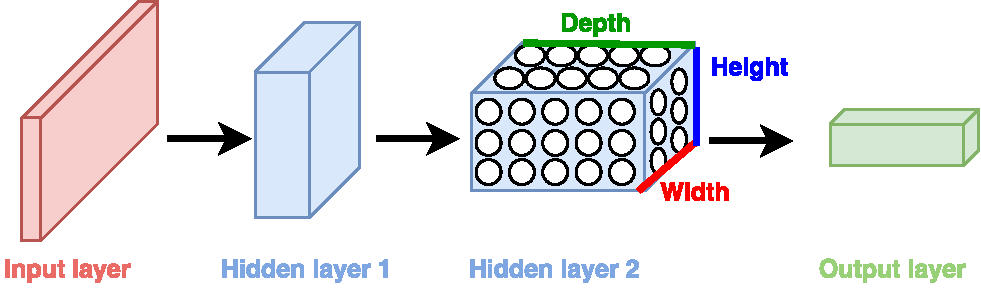
\includegraphics[width=1\textwidth]{Figures/NN_vs_CNN.pdf}
	\caption{A Convolutional Neural Network arranges its neurons in three dimensions (width, height, depth), as visualized in one of the layers. Every layer of a ConvNet transforms the 3D input volume to a 3D output volume of neuron activations. In this example, the red input layer holds the image, so its width and height would be the dimensions of the image, and the depth would be 3 (Red, Green, Blue channels) \cite{CNN_course}}
	\label{fig:NN_vs_CNN}
\end{figure}

\subsubsection*{Layers}
As described earlier a CNN is a combination of layers and every layer transforms one volume of activations to another  through a differentiable function. CNN uses three main types of layers to build the architecture: Convolutional Layer, Pooling Layer, and Fully-Connected Layer (exactly as seen in regular Neural Networks). We will stack these layers to form a full CNN architecture. In reinforcement learning is the pooling layer not used, because they buy translation invariance - the network becomes insensitive to the location of an object in the image.

\subsubsection*{Convolutional Layer}
The Convolutional layer is the main building block of a Convolutional Network that does most of the computational heavy lifting. The convolutional layer consist of a set of learnable filters. every filter is small spatially (along width and height), but extend through the full depth of the input volume. An example of the first layer in a CNN is a filter with size 5x5x3. During the first forward pass it is slide/convolved each filter across the height and width of the input volume and compute dot products between the entries of the filter and the input at any position. As the filter is slide over the input volume it produces a 2-dimensional activation map. The activation map shows the responses of that filter at all spatial position. The network will learn filters that activate when they sees some type of visual feature - such as an edge of some orientation or a patch of some colors. On higher layers the network will learn to see honeycomb or wheel-like patters, so more complete figures. On each convolutional layer it will have an entire set of filters, each layer will produce a separate 2-dimensional activation map. The activation maps will be stacked along the depth dimension and produce the output volume. 

When dealing with high dimensional inputs like images, it is impractical to connect neurons to all neurons in the previous volume. Instead it is smart to connect each neuron to only a local region of the input volume. the spatial extent of this connectivity is a hyperparameter  called the receptive field of the neuron - equivalently this is the filter size. An illustration of the receptive can be seen on \Cref{fig:Respective_field}

\begin{figure}[H]
	\centering
	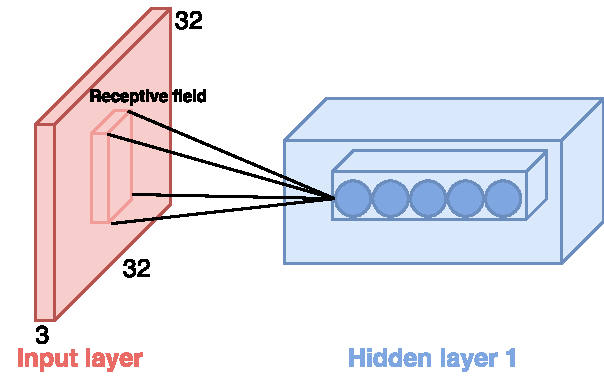
\includegraphics[width=0.7\textwidth]{Figures/Respective_field.pdf}
	\caption{An example input volume in red (e.g. a 32x32x3 CIFAR-10 image), and an example volume of neurons in the first Convolutional layer. Each neuron in the convolutional layer is connected only to a local region in the input volume spatially, but to the full depth (i.e. all color channels). Note, there are multiple neurons (5 in this example) along the depth, all looking at the same region in the input \cite{CNN_course}}
	\label{fig:Respective_field}
\end{figure}


\subsubsection*{Fully connected Layer }
The fully connected layer is a traditional Multi Layer Perceptron. The term “Fully Connected” implies that every neuron in the previous layer is connected to every neuron on the next layer. The output from the convolutional layers represent a high-level features of the input image. The purpose of the Fully Connected layer is to use these features for classifying the input image into various classes. 

Apart from classification fully connected layer is also a cheap way to learn non-linear features from these layers. By combining these features, the classification of the network would be even better. \cite{Fully_Connected_Layer}         